\chapter{Materials and Methods}
\label{chapter:methods}

From now on are presented the data and models used for experiments, and how those nowcasting models were verified. 

\section{Experimental Setup}
\label{section:exp}

In practice, predictions are calculated for BCNN, described in section \ref{section:bcnn}, as well as all models of sections \ref{section:det_model} and \ref{section:prob_model} using all the timestamps contained in the test set described in section \ref{section:data}. Predictions are computed for 36 timesteps, which is equivalent to 3 hours into the future with an interval of 5 minutes. After that, deterministic verification metrics described in section \ref{section:det_metric} are computed for using the predictions of each model, and probabilistic metrics from section \ref{section:prob_metric} are calculated from BCNN and probabilistic models of section \ref{section:prob_model}. Then metrics are averaged over the set for each leadtime of interest. 

In order to make sure that results are valid, all timestamps having any (even a single) observation missing are discarded, and similarly timestamps having any prediction from any model missing are also removed from calculations. Additionally, only pixels where data is present in the predictions of all models are counted in metric calculations. This is accomplished by calculating a common NaN mask using the logical OR operation over NaN values of each model, and subsequently applying that common mask to each prediction.

Regarding probabilistic forecasts, uncertainties present in the data are coming from a diverse set of sources, including both aleatoric and epistemic uncertainties. In order to accurately represent the data distribution resulting from this compound uncertainty, a large ensemble size is needed. Hence, the ensemble size was chosen to be 48 for final models. Verification might be even more reliable with bigger ensembles, but this would be at the expense of too much storage space needed for predictions, which would be very inconvenient. Chosen sizes were deemed to be a good compromise regarding this.

Intermediate results are saved such that predictions are saved in HDF5 archives, in a format where each predicted radar image is a separate dataset in deterministic models, and each ensemble of predicted radar images for a certain leadtime is its separate dataset in ensemble nowcast models. In this storage procedure, predicted float reflectivity values are first compressed into UINT8 with a scale-offset scheme, then thresholded to 0.1 mm/h to facilitate further lossless compression which is finally carried out using GZIP. Trying to reduce the storage space needed is essential because predictions take a very large amount of space on disk. This is a consequence of combining a big number of timestamps, ensemble members and leadtimes for multiple models. Raw metrics do not suffer from the same problem and are saved to disk in a binary Numpy format.  

\subsection{Software and resources}

\begin{figure}
	\centering
	\label{fig:workflow}
	%\missingfigure[figheight=8cm, figwidth=12cm]{Vizualizating the overall workflow with model training, predictions and baselines, metrics, together with used software}
	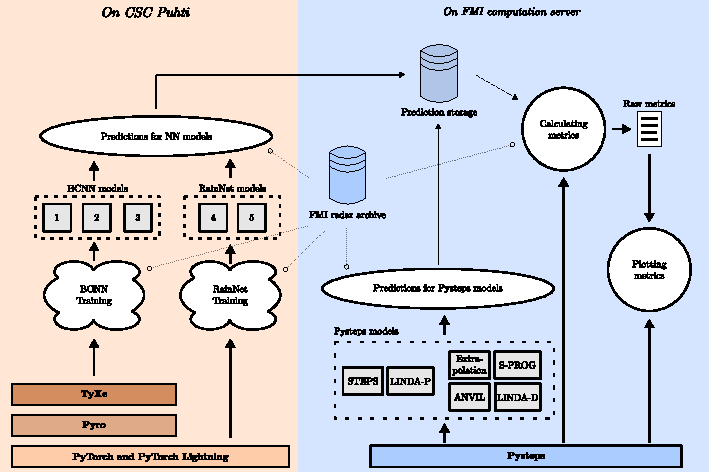
\includegraphics[width=\textwidth]{images/workflow/workflow}
	\caption{Overall workflow used for this work, tied with used libraries for different components.}
\end{figure}

The deep learning models were all implemented using the PyTorch framework and the PyTorch Lightning wrapper \cite{Falcon_PyTorch_Lightning_2019}. These libraries were chosen because of the combined ease of prototyping brought by PyTorch Lightning, and the maturity and flexibility of the parent framework PyTorch. RainNet was ported to PyTorch following the original Tensorflow implementation by Ayzel et al. \cite{Ayzel2020RainNet}. 

As for the implementation of the probabilistic inference mechanisms for Bayesian Neural Networks, choice was made not to implement them by hand, but to rely on the machinery contained in the Probabilistic Programming Language (PPL) Pyro \cite{bingham2018pyro}, which is itself built on top of PyTorch and includes a fully-featured implementation of Stochastical Variational Inference (SVI). In order to facilitate the implementation task, the TyXe package \cite{ritter2021tyxe} was used. TyXe is a library designed to provide an interface simplifying the implementation of Bayesian Neural Networks using PyTorch and Pyro. A few of the reasons why TyXe was chosen are that it permits easily turning existing neural networks into BNNs without having to use hard-coded bayesian layers, and dynamically switching on-and-off the local reparametrization trick and flipout in layers. Some problems encountered include components of TyXe having difficulties working together with PyTorch Lightning abstractions.

Verification experiments and non-deep-learning baseline models were ran and implemented using the open-source library Pysteps \cite{pulkkinen_pysteps_2019}. It provides implementations for all non-deep-learning models described as well as implementation of verification metric primitives used in this work, and tools for their visualization. 

The computational resources from the Finnish IT Center for Science (CSC) were used for GPU intensive tasks such as training and calculating predictions with deep-learning models, and one of FMI's computational servers was used for performing other, more CPU-intensive operations such as predicting with baseline non-deep-learning models and calculating verification metrics. We trained the models on the CSC Puhti supercomputer, using one Nvidia V100 GPU with 32GB of VRAM, 64GB of RAM, and 10 cores from a 2.1 GHz Intel Xeon Gold 6230 CPU. As for the FMI server, it contains 2 Intel Xeon Gold 6138 2.0 GHz CPUs with each 20 cores and 2 threads by core, with 192GB of RAM. 

\section{Dataset and data selection}
\label{section:data}

As input data we use lowest elevation angle radar reflectivity composites with 1km spatial resolution and 5 minute temporal resolution from the Finnish Meteorological Institute, cropped into a 512x512 km region covering southern Finland. The domain and bounding box are illustrated in Figure \ref{fig:domain}. The radar network consists of C-band dual polarization radars. 

Because lowest elevation angle horizontal reflectivity is a good estimator of precipitation at ground level, it is a natural data choice for building a nowcasting model. Radar composites archived from these radar scans are readily available at FMI which facilitated their retrieval for this work. Although the bounding box covering southern Finland did have some data quality issues, it was still deemed to be the best choice, when compared to other candidate datasets such as TAASRAD19 \cite{franch_taasrad19_2020}, as the problems were minor and did not disturb the training process. For example, missing pixels were correctly labeled, which allowed trivial removal of composites with some included. 

Some of the problems with the chosen data are related to lackluster data quality control. Specifically, dual polarization information was not used for the removal of non-meteorological echos, making this removal less accurate. Also, again related to the lack of vertical polarization information, attenuation correction was not performed, meaning that echos originating from behind other strong echos will be attenuated and show as weaker than they really are. This is partly mitigated by having multiple radars in the composite, but even this will not cover all needed scenarios, making this lack of attenuation correction a significant problem. 


%All of these factors contributed to the choice of the data source. 
%such as TAASRAD19 - removed

The dataset was chosen so that at first, a selection of rainy days were chosen as to correspond to the 100 days with the most pixels exceeding a 35 dBZ reflectivity threshold during the summer period spanning from May to September during years 2019, 2020, and 2021. The present threshold was chosen as a value which convective storms usually exceed during their whole lifetime \cite{voormansik_thunderstorm_2017}, as the events that are of the most interest in the context of this work are such convective storms.

This dataset is then cleaned and filtered, after which it is divided into training, validation, and test sets. Cleaning the data involves first going through all timestamps and removing those with either partially or completely missing data. The filtering part consists of removing timestamps with less than 1\% of pixels containing reflectivity values exceeding 20 dBZ. Splitting of data into training, validation, and testing sets is performed by using a block sampling strategy \cite{schultz_can_2021} with 6 hour long blocks to prevent autocorrelation between consecutive radar images from invalidating independence between splits. The final split sizes were 15840 radar images for the training split, 2664 for the validation split, and 2448 for the test split. 

% data transformation to dbz , to RR 
% how was data read: PGM, hdf5 datasets made
% hwo was read : 4 at a time 


%Radar composites are stored as gzip-compressed PGM composite files holding uint8 values, which are converted to reflectivity (dBZ) by applying the relation $\text{pixel\_value}_{\text{dBZ}} = -32 + 0.5 * \text{pixel\_value}_{\text{uint8}}$. 

%When fed into neural networks, the composites are read from HDF5 files as this improves reading speed on distributed storage systems. 

From radar reflectivities, rainrate estimates were calculated using Eq. \ref{eq:z-r} solved for $R$, with empirically determined parameters $A=223$ and $b=1.53$, and $z = 10^{Z / 10}$, giving us a relation of

\begin{equation}
\label{eq:dbz_to_r}
R = (10^{Z / 10} / 223)^{1/1.53}
\end{equation}

for the current data. 

\begin{figure}
	\label{fig:domain}
	\centering
	%\missingfigure[figwidth=12cm, figheight=10cm]{FMI radar domain, bbox}
	\includegraphics[scale=1.2]{images/domain/fmi_domain}
	\caption{FMI radar domain and the chosen bounding box covering southern Finland. The three letter codes identify the radars, inner circles their worst case effective range (usu. during summer), and outer circles their best case effective range (usu. during winter). The lowest level reflectivity composite from the 30th of June 2020 at 00:05:00 is depicted on the right.}
\end{figure} 


\section{Model}

\subsection{The baseline: A U-Net based CNN}
\label{section:rainnet}

For the implementation of a Bayesian Convolutional Network, we use as our base functional model  the same architecture as for RainNet by Ayzel et al. \cite{ayzel_rainnet_nodate}, which is itself heavily inspired by U-Net and SegNet model families. RainNet just like those families adopts a U-shaped encoder-decoder architecture. The encoder is composed of successive pooling and convolutional layers, reducing image sizes passed to the next layer while increasing the number of filters. The decoder part adopts a mirror archictecture of successive upsampling and convolutional layers, increasing the image size while reducing the number of filters. There is 5 levels in the encoder-decoder structure, just like in SegNet. Additionally, there are skip connections from the encoder to the decoder branch, carrying higher-level filter maps through, just like in U-Net. This is done in order not to lose smaller spatial scale details with pooling.  

\begin{figure}[h]
	\label{fig:rainnet}
	%\missingfigure[figwidth=12cm, figheight=8cm]{RainNet architecture diagram with vector graphics}
	\centering
	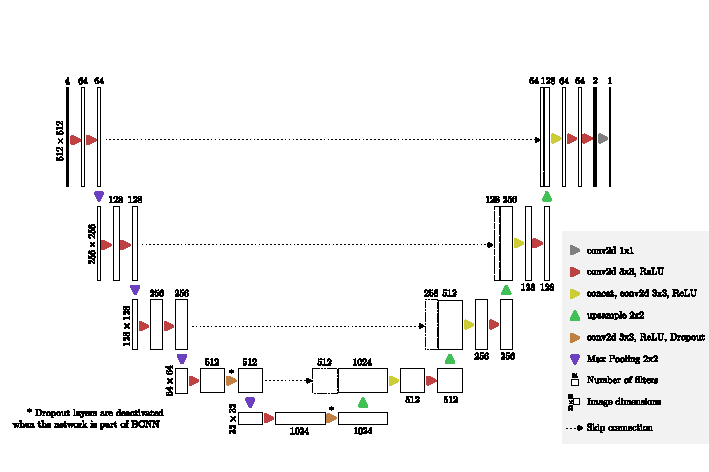
\includegraphics[scale=1]{images/rainnet_arch/rainnet_arch}
	\caption{The functional CNN architecture used for this work, Identical to that of RainNet from Ayzel et al. \cite{ayzel_rainnet_nodate}. \texttt{concat} refers to the concatenation of feature maps along the channel dimension.}
\end{figure}

The convolutional filters have a filter size of 3, with padding designed to preserve image shape, and a stride of one. Finally, the last convolutional layer in the network has a filter size of 1 with no padding, and it is followed by a linear activation output layer, i.e. no (nonlinear) activation function. The network does not contain any fully-connected layers, and in total consists of 31.4M parameters. RainNet works by feeding in 4 consecutive radar images, with the physically speaking temporal dimension represented in the channel dimension of the tensor. As the output of the network, we get one output radar image, representing the next predicted frame. In order to make predictions at further leadtimes, the predictions are fed back to the inputs one-by-one in an iterative process. 

The network is trained by calculating a loss function between observed and predicted radar images. This loss function is originally the LogCosh loss, as described in Ayzel et al.'s paper \cite{ayzel_rainnet_nodate}. In addition to that loss, the use of Multi-Scale Structural Similarity Index (MS-SSIM) \cite{wang_multiscale_2003} as a loss function was also implemented in this work. MS-SSIM is a loss function, originally an 

The rainrates were scaled using a logarithmic transformation $x_{\log} = \ln(x + 0.01)$ for use in the CNN and BCNN models, and they were additionally shifted upwards by a factor of 5 and then scaled down by a factor of 10 to fit into the range of 0 to 1 when using MS-SSIM loss. One benefit of using MS-SSIM instead of Logcosh loss is that MS-SSIM better preserves structural details of predictions such as edges and gradients, which helps with nowcasting higher reflectivity values. This same behaviour however often produces diverging nowcasts, characterized by loss of total precipitation mass and unphysically high precipitation intensities at further leadtimes. The logarithmic transformation of the data is needed because rainrates in themselves are lognormally distributed. This transformation makes them normally distributed, and thus more suitable inputs to neural networks.

The diverging behavior is alleviated by calculating the loss function for nowcasts done over several leadtimes, making the resulting learned network more temporally stable. Hence for training, the predictions are calculated for 6 leadtimes (30 minutes ahead) and the loss is calculated such that each prediction leadtime is weighted equally. Using multiple leadtimes is also implemented for the LogCosh loss function. MS-SSIM was calculated using a data range parameter of 1.0 and equal scale weights of $[0.2, 0.2, 0.2, 0.2, 0.2]$ ordered from smallest to biggest, as opposite to the scaling optimized for visual perception introduced by Wang et al. \cite{wang_multiscale_2003} in the context of using MS-SSIM as a visual quality assessment tool. 

The reason for adopting RainNet as the functional architecture of the Bayesian Neural Network is that compared to for example ConvLSTM based models, it has faster inference without losing much in skill. This is important when building upon a model, especially when having limited resources, as added components make the training and inference slower. 


\subsection{BCNN: a Bayesian extension to RainNet}

\label{section:bcnn}

\fixme{BCNN is a working name, find potentially better name}

BCNN is the Bayesian extension made for this work of the U-Net based architecture described in section \ref{section:rainnet}. In the network, posterior probability distributions of weights and biases are modeled as diagonal Gaussian distributions and optimization is carried out using variants of the Bayes-by-Backprop algorithm described by Blundell et al. (2015) \cite{blundell_weight_2015}, minimizing the ELBO loss function as described in section \ref{section:vi}. Posteriors for all parameters are initialized identically to a mean $\mu$ of 0 and a variance $\sigma$ of 1e-4. Parametrizing the posteriors as Gaussian distributions doubles the number of learnable parameters to 62.8M. The Local Reparametrization Trick (LRT) \cite{kingma_variational_2015} and Flipout \cite{wen_flipout_2018} are both used in an attempt to reduce gradient variance and speed-up optimization. 

As for the prior distribution, two variants are implemented. One being a diagonal Gaussian prior $P(\pmb{w}) \sim \mathcal{N}(0,0.1)$ and the second a Gaussian scale mixture prior as defined in Eq. \ref{eq:gsm}, with $\alpha = 0.5$ and $\sigma_1, \sigma_2 = 0.3, 0.03$. The scale-mixture prior might enable faster initialization and more accurate asymptotic behavior, but the Gaussian prior has more convenient mathematical properties, as it enables calculating KL-divergences in closed form when combined with a Gaussian posterior as in here, using the analytical expression

\begin{equation}
\begin{split}
D_{KL}(q(\mathcal{D}|\pmb{w}) || P(\pmb{w})) =
\frac{1}{2}[\log \frac{|\sigma_P|}{|\sigma_q|}
- d \\
+ (\mu_q - \mu_P)^T \sigma_P^{-1}(\mu_q - \mu_P)
+ tr\{\sigma_P^{-1}\sigma_q\}
]
\end{split}
\end{equation}

where $q$ and $P$ denote the multivariate diagonal posterior and prior, $\mu_q$ and $\mu_P$ their respective means, $\sigma_P$ and $\sigma_q$ their respective standard deviations and  $d$ the identity matrix of the number of dimensions equal to that of the distributions. 

In BCNN, the radar images were scaled between 0 and 1 using the same procedure as described for the MS-SSIM loss function in the context of RainNet in section \ref{section:rainnet}. The data likelihood cost was modeled as Homoscedastic Gaussian likelihood \cite{kendall_what_2017}, defined by 

\begin{equation}
	\mathcal{L}_{Gauss}(y, \hat{y}) = \frac{1}{N} \sum_{i=1}^{N} \frac{1}{2\sigma^2}||y_i - \hat{y}_i||^2 
	+ \frac{1}{2} \log \sigma^2
\end{equation}

where $i = 1 \dots N$ indexes the number of pixels in the images, and $\sigma$ here refers to the observational noise parameter. In homoscedastic gaussian likelihood, aleatoric uncertainty, characterized by $\sigma$ is assumed to be the same for all the data. This parameter can be learned or left constant. The latter is done in the present work, and a value of 0.02 is chosen as a guess, aiming to represent the uncertainty inherent to radar images. 

Multiple procedures for weighting the complexity cost against the likelihood cost, some presented in Section \ref{section:vi}, are implemented. In addition to the equal weighting scheme from Graves et al. \cite{graves_practical_2011} and the batch index dependent scheme from Blundell et al. \cite{blundell_weight_2015}, a scheme reducing the weight of the complexity cost each epoch, defined as $\pi_j = 2^{-j}$, where $j=0,1,\dots$ is the current epoch, is implemented to provide better potential convergence, as the equal weight scheme sometimes provides excessive regularization and the second scheme has problems with converging when using smaller batch sizes as in this work.


\begin{figure}[ht]
	\begin{center}
		\subfigure[Training procedure for the BCNN illustrated. \textbf{Rough first version: cleaning up later with radar imgs/preds over black boxes, alignment, sizes, fonts same everywhere after getting feedback on overall structure}]{
			\label{fig:training}
			%\missingfigure[figwidth=14cm, figheight=5cm]{Training diagram}
			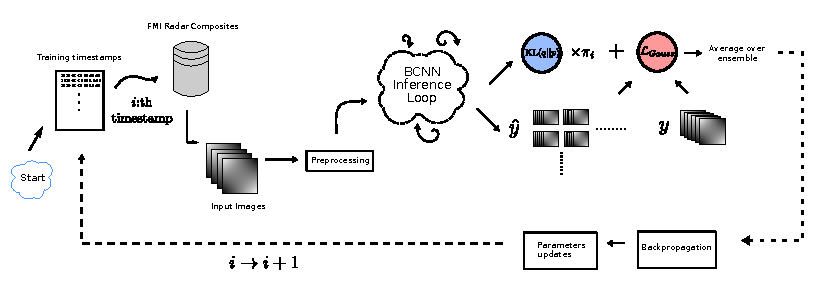
\includegraphics[scale=1]{images/training_diagram/training_diagram.pdf}
		}
		\subfigure[Inference procedure for generating ensemble nowcasts with the BCNN.\textbf{Same comments as above...}]{
			\label{fig:inference}
			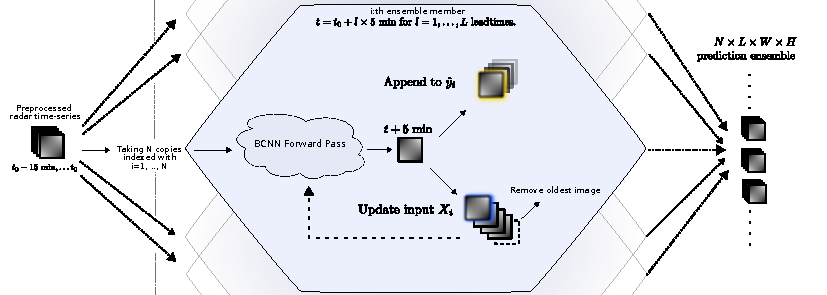
\includegraphics[scale=1]{images/inference_diagram/inference_diagram.pdf}
		}
		\caption{Training and inference procedures}
		\label{fig:training_inference_diagram}
	\end{center}
\end{figure}

The predictions are made by simply performing a forward pass through the network, which samples the parameters and produces a Monte-Carlo (MC) sample, i.e. an ensemble member. Predictions for further leadtimes are made in the same way as with the deterministic RainNet, that is by iteratively re-plugging the output, now a MC sample, into the inputs of the network. It is important to note that stochasticity is preserved because parameters are re-sampled at each step of the iterative prediction. Ensembles are produced by repeating this process multiple times independently, that is, such that one initial MC sample will lead to a no more than a single new MC sample each leadtime. Sampling is done this way to avoid the problem of exponential growth that would appear if each sample at leadtime $t$ would yield more than one sample at leadtime $t+1$. The inference procedure is illustrated in Figure \ref{fig:inference}.

Training is performed such as to train the model to predict on a single leadtime (+5min), and after this performing further training on 6 leadtimes (+30min) until model convergence. This is done in an attempt to speed up model convergence compared to training the model on many leadtimes right from the start. At each training step, one MC sample is drawn from the network and gradients are calculated from its ELBO loss. A diagram illustrating the training process is shown in Figure \ref{fig:training}.

The model selection process is performed hierarchically as follows: Two priors per category, that is a Gaussian prior with $\sigma = 0.1$ and $\sigma = 0.001$, and a Gaussian Scale Mixture (GSM) prior with $\sigma_1, \sigma_2 = 0.3, 0.03$ and   $\sigma_1, \sigma_2 = 0.1, 0.001$ are selected and models are trained with them. Next, the best performing model is selected based on the validation likelihood cost, and it is retrained using the KL-annealing strategy proposed as well as that from Blundell et al. Finally, the best performing model overall is selected for verification against baselines. 

\subsection{Additional Hyper-parameters for NN}
\label{section:hyper}
 Both for RainNet and BCNN, the Adam optimizer is used with an initial learning rate of 1e-04, without any learning rate scheduler. For RainNet, other hyper-parameters were left to their \texttt{torch.optim.Adam} default values, while for BCNN, the momentum parameter $\beta_1$ was increased to $0.95$ to better accommodate the increased stochasticity of SVI compared to non-Bayesian NN \cite{noauthor_svi_nodate}. Early stopping was set with condition that the validation loss does not decrease for 3 epochs for both models. For BCNN, only the likelihood part of the loss was taken into account in the early stopping criterion. 


\section{Verification Baseline Models}

\subsection{Baseline Deterministic Models}
\label{section:det_model}

In order to verify the skill of BCNN, multiple deterministic models were used to produce nowcasts against which those produced by BCNN are compared. First and foremost, the ensemble averages of BCNN are compared against those of RainNet trained with 6 leadtimes, and both LogCosh and MS-SSIM loss, with the configuration outlined in sections \ref{section:rainnet} and \ref{section:hyper}. Although loss functions used for training the network are not comparable, it still is interesting to compare the skill between the classical predictions and Bayesian version ensemble means, as underlying functional architectures are the same.

In addition, predictions were calculated with a few non-deep-learning models introduced in section \ref{section:classic_nowcast}. These are Lagrangian Persistence (extrapolation nowcast) and LINDA-D, the deterministic version of LINDA.

Concerning baseline models other than RainNet, before all predictions, the bounding box is applied, input data is converted to rainrate using Eq. \ref{eq:dbz_to_r} and thresholded at 0.1 mm/h and possible NaN values are set to zero. After predictions are made, these are thresholded at 0.1 mm/h and converted to back to reflectivities by first using Eq. \ref{eq:z-r} with parameters $A$ and $b$ stated in section \ref{section:data} and then converting Z to dBZ for storage. When predictions are read for metric calculation, they are once again converted to rainrate before metric calculation.

Both extrapolation and LINDA-D, as well as models described in section \ref{section:prob_model} use Lucas-Kanade optical flow for advection field estimation with default parameters and four input frames with field interpolation. These models also perform advection using Pysteps' Semi-Lagrangian backward scheme, using cubic interpolation, again with other parameters left to default values. LINDA-D has stochastic  perturbations set off with the \texttt{add\_perturbations} flag and otherwise uses default parameters. 


\subsection{Baseline Probabilistic Models}
\label{section:prob_model}

Probabilistic skill verification was performed against STEPS and LINDA-P. The former was chosen as it is a well-established and broadly used model offering good performance for a relatively low inference cost of 1-2 minutes to produce a 3 hours nowcast of 24-48 ensemble members on a modern CPU for a domain of 512x512 pixels \cite{pulkkinen_pysteps_2019}. It thus makes sense to want BCNN to perform at least on the same level as STEPS, considering that the time required for inference with it might not be much lower than that. LINDA-P, also known as the probabilistic variant of LINDA, is computationally more expensive but represents the state-of-the-art in terms of probabilistically predicting localized high-intensity rainfall. Consequently, LINDA-P makes for an interesting benchmark for those cases. 

The same preprocessing and postprocessing pipelines as for deterministic cases (section \ref{section:det_model}) are used with baseline probabilistic models. Also, the same optical flow and extrapolation parameters are used, and again, Pysteps 1.6.1 default values for methods are used unless stated otherwise. 

As stated in section \ref{section:exp}, probabilistic nowcast produce 48 ensemble members. STEPS has parameters set to match the input data, that is \texttt{km\_per\_pixel} is 2.0 and \texttt{timestep} is 5.0, also \texttt{R\_thr} is set to -10. LINDA-P has the same parameters as LINDA-D, except that naturally stochastic perturbations are set to \texttt{True} with the \texttt{add\_perturbations} flag.

\section{Verification Visualizations and Metrics}

\subsection{Deterministic Prediction skill evaluation metrics}
\label{section:det_metric}

Deterministic prediction skill scores were calculated in order to compare the raw predictive skill of ensemble nowcasts to the skill of deterministic models. Such comparison is an important facet of verification as low skill in deterministic scores would even for an otherwise competent model mean that it would benefit from being complemented by a stronger deterministic model. In the case of ensemble nowcasting, Deterministic scores were calculated for ensemble means. Implemented deterministic metrics are divided into four different categories, roughly complementing each others. These are continuous, categorical, and spatial scores, as well as radially-averaged power spectral density.  

Continuous scores scores are as their name suggests distance metrics used for the evaluation of continuously valued predictions, i.e. regression tasks. The continuous scores used are Mean Error (ME) and Mean Absolute Error (MAE). ME is defined as 

\begin{equation}
	\text{ME} = \frac{1}{N}\sum_{i=1}^{N} y_i - \hat{y}_i,
\end{equation}

where we sum over the $i=1,\dots,N$ pixels in the radar image, $y$ denotes ground truth and $\hat{y}$ the prediction made. The principal utility of Mean Error is detection whether predictions are biased towards too low or too high rainrates at a certain point in time. On the other hand, 

\begin{equation}
	\text{MAE} = \frac{1}{N}\sum_{i=1}^{N} |y_i - \hat{y}_i|,
\end{equation}

only cares about the magnitude of the errors in predictions by taking the absolute value, so it gives an idea of the prediction skill over the images \textit{on average}. Nevertheless, this is not enough to accurately assess the skill of a nowcast method, because not all pixels are equally important, as most of them have no rain or very low rainrates that are not interesting to predict. Additionally, A poor forecast may have good MAE and vice versa. To illustrate this, a forecast failing to predict localized intense rainfall, but otherwise accurately capturing light rainfall over large areas will usually have a small MAE but will have low operational usefulness.


\begin{wraptable}{r}{0.6\textwidth}
	\centering
		\begin{tabular}{@{}|c|c|c|@{}}
			
			\toprule
			\textit{\begin{tabular}[c]{@{}c@{}}Precipitation\\ is ...\end{tabular}} &
			\multicolumn{1}{l|}{\textbf{Observed}} &
			\textbf{\begin{tabular}[c]{@{}c@{}}Not\\ observed\end{tabular}} \\ \midrule
			\textbf{Predicted} &
			\cellcolor[HTML]{D9FFD9}\begin{tabular}[c]{@{}c@{}}TP\\ (Hits)\end{tabular} &
			\cellcolor[HTML]{FFCAB1}\begin{tabular}[c]{@{}c@{}}FP\\ (False Alarms)\end{tabular} \\ \midrule
			\textbf{\begin{tabular}[c]{@{}c@{}}Not\\ predicted\end{tabular}} &
			\cellcolor[HTML]{FFCAB1}\begin{tabular}[c]{@{}c@{}}FN\\ (Misses)\end{tabular} &
			TN \\ \bottomrule
		\end{tabular}
	\caption{Contingency table of categories used. Alternative nomenclature is shown in parentheses.}
	\label{table:contingency}
\end{wraptable}


This limited utility of continuous scores serves as a motivation to introduce categorical scores. These are based on the principle of comparing the presence or absence of a rain event in observations and predictions as defined by having a pixel exceeding a threshold value $R_{\text{THR}}$. The categorical scores are defined by dividing events into four categories, that are true positives (TP), i.e rain events that were correctly predicted, true negatives (TN), i.e. lack of rain event that was correctly predicted, false negatives (FN), i.e. rain that wasn't successfully predicted, and false positives (FP), i.e rain that was erroneously predicted. These categories and their relations are illustrated in Table \ref{table:contingency}. Scores derived from those quantities that were used are probability of detection (POD) \cite{schaefer_critical_1990} defined as

\begin{equation}
	\text{POD} = \frac{\text{TP}}{\text{TP}+\text{FN}}
\end{equation} 

, which simply tells the probability that an event really occuring is correctly predicted. Next, false alarm rate (FAR) \cite{schaefer_critical_1990} is calculated as 

\begin{equation}
	\text{FAR} = \frac{\text{FP}}{\text{TP}+\text{FP}}
\end{equation}

which reversely indicates the percentage of positively predicted events not actually happening. Critical success index (CSI) \cite{schaefer_critical_1990}, which is defined as 

\begin{equation}
	\text{CSI} = \frac{\text{TP}}{\text{TP}+\text{FN}+\text{FP}}
\end{equation}

is computed and aims to generally assess the performance of the forecast by taking the proportion of correct positive event predictions out of critically important cases, that is those excluding true negatives but including both false alarms (FP) and misses (FN). Lastly, the equitable threat score (ETS) \cite{hogan_equitability_2010} is defined as  

\begin{equation}
\begin{split}
\text{ETS} = \frac{\text{TP} - rnd}{\text{TP}+\text{FN}+\text{FP}- rnd}, \\
\text{where } rnd = \frac{(\text{TP}+\text{FN})(\text{TP}+\text{FP})}{\text{TP}+\text{FN}+\text{FP}+\text{TN}}
\end{split}
\end{equation}

was computed. ETS aims to improve CSI assessment of forecast skill, by attempting to estimate the amount of random TP among the prediction using the term $rnd$, and remove that number of data points from the calculations.

The $R_{\text{thr}}$ thresholds chosen for the performing verification are 0.5, 1.0, 5.0, 10.0, 20.0, and 30.0 mm/h. 0.5 mm/h corresponds to very light rainfall and should be easy to predict, while higher thresholds like 20.0 and 30.0 mm/h correspond to very heavy rainfall, which are very difficult to predict even for short leadtimes.

In addition to evaluating prediction skill above rainrate thresholds, it is also important to be able to evaluate the nowcast at multiple scales. The reason for this is that bigger scales have more predictability, and so predicting smaller scales is more difficult while also being of high importance in the context of heavy localized rainfall. 

%in fss, we can determine a threshold for acceptable skill to determine the scale at which nowcasts are good wrt lt 

As such, spatial verification scores, namely Fraction Skill Score (FSS) \cite{roberts_scale-selective_2008} and intensity-scale verification using FSS are added to the panoply of metrics used. FSS is a verification metric aiming to estimate the prediction skill above a certain threshold at different spatial scales. It works by calculating a binary threshold exceedance map for forecasts and observations, averaging it over gaussian windows of different lengths representing scales, and calculating for each of those a Mean Squared Error (MSE) skill score relative to a reference low-skill forecast \cite{roberts_scale-selective_2008}. Calculating spatial verification scores for a matrix of rainrate intensity threshold and spatial scale is known as intensity-scale verification. Such verification was performed using FSS for thresholds of 0.5, 1.0, 5.0, 10.0 and 20.0 and 30.0 mm/h, as well as spatial scales of 1, 2, 4, 8, and 16 km. 

Last but not least, the ability to maintain small-scale details as the forecast leadtime increases is related to the skill of the nowcast with regards to the spatial scale. Failure in maintaining those details will results in low skill at small scales and a blurred forecast demonstrated by a dip in nowcast small-frequency power spectral density. Hence the last deterministic verification metric chosen is Radially-Averaged Power Spectral Density (RAPSD). This metric as its name suggests provides a way of calculating power spectral densities for 2D images such as nowcasts, independently of direction. RAPSD characterizes the amount and type of blurring occurring in deep-learning based models verified. It is calculated for 15, 30, 60, and 180 minute leadtimes.
 
\fixme{fix leadtimes, threshs, scales, before submit}

\subsection{Visual Evaluation of nowcast predictive uncertainty and Skill}

In order to visually assess ensemble nowcasts, ensemble mean and standard deviations of nowcasts were plotted and compared to radar observations. In addition, rainrate exceedance probability estimations for the ensemble were plotted for thresholds of 0.5 and 5.0 mm/h. Leadtimes chosen for these visualizations included 5, 15, 30, and 60 minutes or alternatively 5, 60, 120, and 180 minutes for studying longer less skillful prediction time-scales.

These visualizations were made for two distinct cases, one containing purely convective rainfall and the other containing a mix of stratiform and convective rainfall. This heterogeneous set serves to assess differences in the developed method with regards to the rainfall type, knowing that convective events are notoriously harder to predict.

\subsection{Probabilistic Prediction skill evaluation metrics}

\label{section:prob_metric}
Deterministic verification scores are not enough to accurately assess ensemble forecast skill, because the advantage brought by ensembles does not lie in their mean value, but rather in the breath and quality of their distributions, allowing to weight in multiple possible scenarios. Consequently, specialized metrics designed to assess probabilistic forecasts are needed. 
For this work, four different probabilistic metrics are used for verification. These are the Continuous Ranked Probability Score (CRPS), rank histograms, reliability diagrams, and Receiver operating characteristic (ROC) curves. 

CRPS is a metric generalizing MAE for probabilistic forecast. It is defined as 

\begin{equation}
	\text{CRPS}(F,x) = \int_{-\infty}^{\infty} (F(y) - \mathds{1}(x \geq y))^2 dy
\end{equation}

where $F$ is the forecast cumulative density function (CDF) and $\mathds{1}(x \geq y)$ is the empirical CDF of the observation $x$. CRPS aims thus to represent the distance between those cumulative distributions as a proxy to estimate ensemble forecast skill. 

A rank histogram is a measure that from the rank of the radar observation among ensemble members, builds a histogram. For each pixel, the rank is determined and and a bin is incremented accordingly. The shape of the histogram is indicative of  whether the spread of the ensemble is representative of the true spread of observations. Variability in the ensemble equal to the uncertainty of observations would make a flat histogram. A convex histogram would mean that ensemble spread under-estimates true uncertainty, whereas a concave histogram would mean that uncertainty is over-estimated, that is that the ensemble is more uncertain that it should be. Furthermore, skewness of the histogram gives a hint on whether there is any kind of bias in the predictions of the ensemble. This goes a step further than ME, as it does not simply tell the average error, but estimates its distribution in a sense. 


ROC curves \cite{mason1982model} are a verification method assessing the ability of a forecast to discern between positive and negative events, that is in the present case pixels with or without exceedance of a particular rainrate threshold. This is accomplished by keeping track of false alarm rates (FAR) against probability of detection (POD) of an event. Probabilities are divided into a certain number of bins over which corresponding FAR are averaged, and a curve is formed. A random forecast corresponding to no skill corresponds to a line, and an increasing area under the curve indicates better discernment ability. 

A reliability diagram presents observed relative frequencies of events (rainrates exceeding a certain threshold value) against their forecast probabilities. When these two values are close to each others, the forecast is said to be reliable. This means that a skillful forecast is defined by being close to the line of equality to observed relative frequencies for all forecast probabilities output by the model. 

ROC curves are conditioned on observation of an event, while reliability diagrams are conditioned on its forecast. Because of this they complement each others well in the evaluation of ensemble prediction skill. For probabilistic metrics, the same rain intensity thresholds as in deterministic metrics, namely 0.5, 1.0, 5.0, 10.0, 20.0, and 30.0 mm/h are used. CRPS is calculated for the whole 36 leadtimes covering 3 hours, while other metrics are calculated for leadtimes of 15, 30, 60, 120, and 180 minutes. 

\fixme{Fix LTs, thresholds at the end, after experiments are finished}

 All of the scores described in sections \ref{section:det_metric} and \ref{section:prob_metric} complement each others, and forecast skill is thus estimated as a combination of them, as no score is able to capture all of the facets of a great nowcast. 
 

